\clearpage
\section*{Problem 1}
\begin{enumerate}[a)]
    \item Tag 1 tells the compiler to allocate 2-bytes to the stack and treat this value as a 16-bit signed integer.\\
    Tag 2 tells the compiler to allocate a variable amount of bytes to the stack. This value would be treated as an address to FILE data. Additionally, Tag 2 also allocates space on the heap for the File itself\\
    Tag 3 will send the formatted string to the file output stream.
    \item Code compilation with output
    \begin{figure}[h]
        \centering
        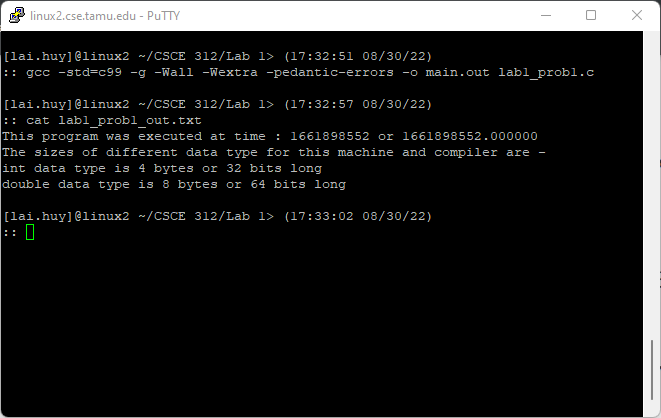
\includegraphics[width=10cm]{Images/1b.png}
        \caption{Compilation and Output}
    \end{figure}
    
    \item The data type of ``timeval'' is a signed 16-byte integer. It indicates the number of second that have elapsed since 00:00:00 on January 1, 1970, Coordinated Universal Time.
\end{enumerate}